\documentclass{beamer}

\usepackage{xcolor}
\usepackage{color}
\usepackage{graphicx}
\def\xcolorversion{2.00}
\def\xkeyvalversion{1.8}
\setbeamersize{text margin left=0pt,text margin right=0pt}

\makeatletter
\newcommand*\bigcdot{\mathpalette\bigcdot@{.9}}
\newcommand*\bigcdot@[2]{\mathbin{\vcenter{\hbox{\scalebox{#2}{$\m@th#1\bullet$}}}}}
\makeatother

\usepackage{TIKZ_Macra}
\usepackage{xparse}
\usepackage[utf8]{inputenc}
\usepackage[T1]{fontenc}

\useinnertheme[shadow=true]{rounded}
\setbeamercolor{block title}{use=structure,fg=structure.fg,bg=structure.fg!30!bg}
\setbeamercolor{block body}{parent=normal text,use=block title,bg=block title.bg!50!bg}
\setbeamercolor{block title example}{use=example text,fg=example text.fg,bg=example text.fg!30!bg}
\setbeamercolor{block body example}{parent=normal text,use=block title example,bg=block title example.bg!50!bg}

\usepackage[most]{tcolorbox}
\usepackage{lmodern}
\usepackage{mathtools}
\usepackage{amsfonts}
\usepackage{amssymb}
\usepackage{latexsym}
\usepackage{hyperref}
\usepackage{changepage}

\newtcbox{\mybox}{blank, on line, opacitytext=0.5}

\usepackage{Moje_makra}
\usepackage{Moje_Zmienne}
\usepackage{Zbiory_i_konfiguracje}
\usepackage{Complexity}
\usepackage{Sieci}

\newcommand{\Bool}{\mathbb{B}}
\newcommand{\Sat}{\mathsf{Sat}}
\newcommand{\PreStates}{\mathsf{Pre}}
\newcommand{\Paths}{\mathsf{Paths}}
\newcommand{\Sub}{\mathsf{Sub}}
\newcommand{\EF}{\mathsf{EF}}
\newcommand{\AF}{\mathsf{AF}}
\newcommand{\EG}{\mathsf{EG}}
\newcommand{\AG}{\mathsf{AG}}
\newcommand{\EX}{\mathsf{EX}}
\newcommand{\AX}{\mathsf{AX}}
\newcommand{\EU}{\mathsf{E}\,\mathsf{U}}
\newcommand{\AU}{\mathsf{A}\,\mathsf{U}}

\begin{document}

\begin{frame}[fragile]{}
\Margines{
\begin{center}
  {\huge Theory of Concurrency}\medskip

  {\large Lecture 2: Temporal logics}\medskip

  Piotr Hofman
\end{center}
}
\end{frame}

\begin{frame}{Plan}
\Margines{
\begin{enumerate}
  \item Why automata are useful, but inconvenient as specifications.
  \item Linear temporal logic (LTL): syntax and semantics.
  \item LTL model checking via \Buchi\ automata.
  \item Branching-time logics: CTL and CTL*.
  \item CTL model checking by labelling states.
  \item Why LTL and CTL are not comparable.
\end{enumerate}
}
\end{frame}

\begin{frame}{Specification of properties}
\Margines{
\begin{block}{From automata to logic}
Automata over infinite words are a precise way to specify behaviours, but they are often not convenient to write directly.
\end{block}

\begin{block}{Goal}
We want a small query language for properties of runs, for example:
\begin{itemize}
  \item an error never happens;
  \item every request is eventually answered;
  \item a process is never permanently ignored;
  \item from every state there is a possible recovery.
\end{itemize}
\end{block}

\begin{block}{Main distinction}
LTL speaks about one linear behaviour at a time. CTL also speaks about branching choices between possible futures.
\end{block}
}
\end{frame}

\begin{frame}{Where formulas are evaluated}
\Margines{
\begin{block}{Kripke structure}
Let
\[
  M=(S,I,R,L)
\]
be a Kripke structure over atomic propositions \(\AProp\), where \(R\) is left-total.
\end{block}

\begin{block}{Paths, traces and alphabet}
An infinite path from \(s_0\) is a sequence
\[
  \pi=s_0s_1s_2\ldots
\]
such that \((s_i,s_{i+1})\in R\) for every \(i\geq 0\). Its trace is
\[
  L(s_0)L(s_1)L(s_2)\ldots \in (2^{\AProp})^\omega.
\]
Thus the alphabet for LTL over \(M\) is \(\Sigma=2^{\AProp}\).
\end{block}
}
\end{frame}

\begin{frame}{LTL: syntax}
\Margines{
\begin{block}{Definition}
An LTL formula \(\varphi\) over \(\AProp\) is generated by
\[
\varphi ::= \mathsf{true} \mid p \mid \neg \varphi \mid
             \varphi_1\land \varphi_2 \mid X\varphi \mid
             \varphi_1\,U\,\varphi_2,
\]
where \(p\in\AProp\).
\end{block}

\begin{block}{Temporal operators}
\begin{itemize}
  \item \(X\varphi\): \(\varphi\) holds in the \emph{next} position.
  \item \(\varphi_1 U \varphi_2\): \(\varphi_1\) holds \emph{until} \(\varphi_2\) holds.
\end{itemize}
\end{block}

\begin{block}{Derived operators}
\[
F\varphi \;\equiv\; \mathsf{true}\,U\,\varphi,
\qquad
G\varphi \;\equiv\; \neg F\neg\varphi.
\]
\(F\varphi\) means eventually \(\varphi\), and \(G\varphi\) means always \(\varphi\).
\end{block}
}
\end{frame}

\begin{frame}{LTL: semantics on words}
\Margines{
Let \(w=w_0w_1w_2\ldots\in(2^{\AProp})^\omega\). We write \(w,i\models\varphi\) if \(\varphi\) holds at position \(i\).

\begin{block}{Boolean part}
\begin{align*}
 w,i &\models \mathsf{true},\\
 w,i &\models p &&\text{iff } p\in w_i,\\
 w,i &\models \neg\varphi &&\text{iff } w,i\not\models\varphi,\\
 w,i &\models \varphi\land\psi &&\text{iff } w,i\models\varphi \text{ and } w,i\models\psi.
\end{align*}
\end{block}

\begin{block}{Temporal part}
\begin{align*}
 w,i &\models X\varphi &&\text{iff } w,i+1\models\varphi,\\
 w,i &\models \varphi U\psi &&\text{iff there is } j\geq i \text{ such that } w,j\models\psi \\
 &&&\text{and } w,k\models\varphi \text{ for all } i\leq k<j.
\end{align*}
\end{block}

We write \(w\models\varphi\) for \(w,0\models\varphi\).
}
\end{frame}

\begin{frame}{LTL: semantics on a path}
\Margines{
\begin{center}
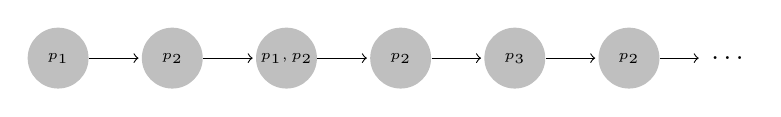
\begin{tikzpicture}[shorten >=1pt,->]
  \tikzstyle{vertex}=[circle,fill=black!25,minimum size=22pt,inner sep=1pt]
  \foreach \name/\lab/\x in {0/{p_1}/0,1/{p_2}/1.45,2/{p_1,p_2}/2.9,3/{p_2}/4.35,4/{p_3}/5.8,5/{p_2}/7.25}
    \node[vertex] (G-\name) at (\x,0) {\tiny $\lab$};
  \node[] (dots) at (8.5,0) {$\ldots$};
  \foreach \from/\to in {0/1,1/2,2/3,3/4,4/5}
    \draw (G-\from) -> (G-\to);
  \draw (G-5) -> (dots);
\end{tikzpicture}
\end{center}

\begin{itemize}
  \item \(p_1\) holds at position \(0\).
  \item \(p_2\) does not hold at position \(0\), but \(Xp_2\) holds.
  \item \(XX(p_1\land p_2)\) holds.
  \item \(Fp_3\) holds, because \(p_3\) holds at position \(4\).
  \item \(G(p_1\lor p_2)\) does not hold, because position \(4\) has only \(p_3\).
  \item \((p_1\lor p_2)Up_3\) holds.
\end{itemize}
}
\end{frame}

\begin{frame}{LTL: satisfaction in a Kripke structure}
\Margines{
\begin{block}{Path satisfaction}
For an infinite path \(\pi=s_0s_1s_2\ldots\), define
\[
  \pi\models\varphi
  \quad\text{iff}\quad
  L(s_0)L(s_1)L(s_2)\ldots \models\varphi.
\]
\end{block}

\begin{block}{Model satisfaction}
For a Kripke structure \(M=(S,I,R,L)\), we write
\[
  M\models\varphi
\]
if every infinite path starting in an initial state satisfies \(\varphi\).
\end{block}

\begin{block}{Important convention}
In model checking, LTL is usually interpreted universally over paths:
\[
  M\models\varphi
  \quad\Longleftrightarrow\quad
  \trace{M}\subseteq \words{\varphi}.
\]
\end{block}
}
\end{frame}

\begin{frame}{Examples: reading LTL formulas}
\Margines{
\begin{itemize}
  \item \(Fp\): eventually \(p\) holds.
  \item \(Gp\): \(p\) holds at every position.
  \item \(GFp\): \(p\) holds infinitely often.
  \item \(FGp\): from some point on, \(p\) always holds.
  \item \(G(req\rightarrow Fack)\): every request is eventually acknowledged.
  \item \(G(crit\rightarrow \neg error)\): whenever the system is in a critical section, no error holds.
  \item \(G(try_i\rightarrow F enter_i)\): process \(i\) is not starved.
\end{itemize}

\begin{block}{Safety and liveness intuition}
\begin{itemize}
  \item Safety: ``nothing bad happens'', e.g. \(G\neg error\).
  \item Liveness: ``something good eventually happens'', e.g. \(G(req\rightarrow Fack)\).
\end{itemize}
\end{block}
}
\end{frame}

\begin{frame}{Examples: exercises}
\Margines{
Express the following properties in LTL.

\begin{enumerate}
  \item Eventually there is a state in which \(p_2\) holds.\par
  \visible<2->{\[Fp_2\]}

  \item Every state along the path satisfies \(p_2\).\par
  \visible<3->{\[Gp_2\]}

  \item If \(p_2\) holds at position \(2\), then \(p_1\lor p_3\) holds at position \(4\).\par
  \visible<4->{\[XXp_2\rightarrow XXXX(p_1\lor p_3)\]}

  \item If \(p_1\) holds in some state, then \(p_2\) holds later.\par
  \visible<5->{\[G(p_1\rightarrow Fp_2)\]}
\end{enumerate}
}
\end{frame}

\begin{frame}{From LTL to \Buchi\ automata}
\Margines{
\begin{block}{Lemma}
For every LTL formula \(\varphi\) one can construct a \Buchi\ automaton \(B_\varphi\) over alphabet \(\Sigma=2^{\AProp}\) such that
\[
  \lang{B_\varphi}=\words{\varphi}.
\]
The automaton has size exponential in \(\abs{\varphi}\) in the worst case.
\end{block}

\begin{block}{Consequences}
LTL formulas define \(\omega\)-regular languages. Therefore, LTL verification can be reduced to emptiness of \Buchi\ automata.
\end{block}

\begin{block}{Warning}
The translation is not the main topic of this lecture. We use it as a black box.
\end{block}
}
\end{frame}

\begin{frame}{LTL model checking}
\Margines{
\begin{block}{Question}
Given a Kripke structure \(M\) and an LTL formula \(\varphi\), decide whether
\[
  M\models\varphi.
\]
\end{block}

\begin{block}{Automata-theoretic algorithm}
\begin{enumerate}
  \item Build a \Buchi\ automaton \(A_M\) such that
  \[
    \lang{A_M}=\trace{M}.
  \]
  \item Build a \Buchi\ automaton \(B_{\neg\varphi}\) such that
  \[
    \lang{B_{\neg\varphi}}=\words{\neg\varphi}.
  \]
  \item Check whether
  \[
    \lang{A_M}\cap \lang{B_{\neg\varphi}}=\emptyset.
  \]
\end{enumerate}
\end{block}
}
\end{frame}

\begin{frame}{Why use the negation?}
\Margines{
\begin{block}{Counterexample search}
The system violates \(\varphi\) iff it has an execution satisfying \(\neg\varphi\):
\[
  M\not\models\varphi
  \quad\Longleftrightarrow\quad
  \trace{M}\cap \words{\neg\varphi}\neq\emptyset.
\]
\end{block}

\begin{block}{Interpretation}
A nonempty intersection gives a counterexample trace:
\[
  \text{system behaviour} \quad + \quad \text{violation of the formula}.
\]
\end{block}

\begin{block}{Nonemptiness of a \Buchi\ automaton}
A \Buchi\ automaton is nonempty iff it has a reachable accepting cycle.

a finite prefix reaches the cycle, and then the cycle is repeated forever.
\end{block}
}
\end{frame}

\begin{frame}{Product construction for LTL model checking}
\Margines{

\vspace{-5mm}

\begin{block}{Product automaton}
Construct the synchronous product
\[
  A_M \times B_{\neg\varphi}.
\]
A state of the product remembers both a state of the system and a state of the automaton for \(\neg\varphi\).
\end{block}

\begin{block}{Acceptance}
The product accepts exactly the traces that are both possible behaviours of \(M\) and violations of \(\varphi\):
\[
  \lang{A_M\times B_{\neg\varphi}}
  = \trace{M}\cap\words{\neg\varphi}.
\]
\end{block}

\begin{block}{Decision procedure}
\[
  M\models\varphi
  \quad\Longleftrightarrow\quad
  A_M\times B_{\neg\varphi}\text{ is empty.}
\]
\end{block}
}
\end{frame}

\begin{frame}{Limitations of LTL}
\Margines{
\begin{block}{LTL is linear-time}
LTL formulas speak about individual infinite paths. They can say what must happen along every possible execution.
\end{block}

\begin{block}{But some properties are branching-time}
For example:
\begin{itemize}
  \item from every reachable state there exists a recovery path;
  \item whenever an error occurs, there is some continuation that repairs it;
  \item a scheduler has a possible strategy to avoid deadlock.
\end{itemize}
\end{block}

\begin{block}{Need}
To express such properties directly, we introduce explicit path quantifiers:
\[
A = \text{for all paths}, \qquad E = \text{there exists a path}.
\]
\end{block}
}
\end{frame}

\begin{frame}{CTL: syntax}
\Margines{
\begin{block}{Definition}
A CTL formula \(\Phi\) over \(\AProp\) is generated by
\[
\Phi ::= \mathsf{true} \mid p \mid \neg\Phi \mid \Phi_1\land\Phi_2
       \mid EX\Phi \mid AX\Phi
       \mid E(\Phi_1 U \Phi_2) \mid A(\Phi_1 U \Phi_2),
\]
where \(p\in\AProp\).
\end{block}

\begin{block}{Derived CTL operators}
\begin{align*}
EF\Phi &\equiv E(\mathsf{true} U \Phi),&
AF\Phi &\equiv A(\mathsf{true} U \Phi),\\
EG\Phi &\equiv \neg AF\neg\Phi,&
AG\Phi &\equiv \neg EF\neg\Phi.
\end{align*}
\end{block}

\begin{block}{Reading}
\(A\) and \(E\) quantify over paths starting in the current state.
\end{block}
}
\end{frame}

\begin{frame}{CTL: semantics}
\Margines{
CTL formulas are evaluated in states of a Kripke structure \(M=(S,I,R,L)\). We write \(M,s\models\Phi\).

\begin{block}{Boolean part}
\begin{align*}
M,s &\models p &&\text{iff } p\in L(s),\\
M,s &\models \neg\Phi &&\text{iff } M,s\not\models\Phi,\\
M,s &\models \Phi\land\Psi &&\text{iff } M,s\models\Phi \text{ and } M,s\models\Psi.
\end{align*}
\end{block}

\begin{block}{Next operators}
\begin{align*}
M,s &\models EX\Phi &&\text{iff for some } s'\text{ with }(s,s')\in R,\ M,s'\models\Phi,\\
M,s &\models AX\Phi &&\text{iff for every } s'\text{ with }(s,s')\in R,\ M,s'\models\Phi.
\end{align*}
\end{block}
}
\end{frame}

\begin{frame}{CTL: until semantics}
\Margines{
\begin{block}{Existential until}
\[
M,s\models E(\Phi U\Psi)
\]
iff there exists a path \(s=s_0s_1s_2\ldots\) and an index \(j\geq0\) such that:
\begin{itemize}
  \item \(M,s_j\models\Psi\),
  \item \(M,s_i\models\Phi\) for every \(0\leq i<j\).
\end{itemize}
\end{block}

\begin{block}{Universal until}
\[
M,s\models A(\Phi U\Psi)
\]
iff for every path \(s=s_0s_1s_2\ldots\) there is an index \(j\geq0\) such that:
\begin{itemize}
  \item \(M,s_j\models\Psi\),
  \item \(M,s_i\models\Phi\) for every \(0\leq i<j\).
\end{itemize}
\end{block}

\begin{block}{Model satisfaction}
\(M\models\Phi\) iff \(M,s\models\Phi\) for every \(s\in I\).
\end{block}
}
\end{frame}

\begin{frame}{CTL examples}
\Margines{
\begin{itemize}
  \item \(AG\neg error\): no error is reachable.
  \item \(AG(req\rightarrow AF ack)\): after every request, acknowledgement is inevitable.
  \item \(AG(req\rightarrow EF ack)\): after every request, acknowledgement is still possible.
  \item \(EF deadlock\): there exists a path to a deadlock state.
  \item \(AG EF reset\): from every reachable state, reset is still reachable.
  \item \(EG\neg error\): there exists an infinite path avoiding error forever.
\end{itemize}

\begin{block}{Important contrast}
\[
AG(req\rightarrow AFack)
\quad\text{is stronger than}\quad
AG(req\rightarrow EFack).
\]
The first says that acknowledgement is unavoidable; the second says that it is possible.
\end{block}
}
\end{frame}

\begin{frame}{CTL model checking: idea}
\Margines{
\begin{block}{Input}
A finite Kripke structure \(M=(S,I,R,L)\) and a CTL formula \(\Phi\).
\end{block}

\begin{block}{Output}
The set
\[
  \Sat(\Phi)=\{s\in S\mid M,s\models\Phi\}.
\]
Then \(M\models\Phi\) iff \(I\subseteq \Sat(\Phi)\).
\end{block}

\begin{block}{Method}
Compute \(\Sat(\Psi)\) bottom-up for all subformulas \(\Psi\in\Sub(\Phi)\). Each temporal operator becomes a graph problem on \(M\).
\end{block}
}
\end{frame}

\begin{frame}{CTL model checking: Boolean and next operators}
\Margines{
Let \(X\subseteq S\). Define the predecessor operator
\[
\PreStates(X)=\{s\in S\mid \exists s'\in X:(s,s')\in R\}.
\]

\begin{block}{Basic cases}
\begin{align*}
\Sat(p) &= \{s\in S\mid p\in L(s)\},\\
\Sat(\neg\Phi) &= S\setminus \Sat(\Phi),\\
\Sat(\Phi\land\Psi) &= \Sat(\Phi)\cap\Sat(\Psi).
\end{align*}
\end{block}

\begin{block}{Next operators}
\begin{align*}
\Sat(EX\Phi) &= \PreStates(\Sat(\Phi)),\\
\Sat(AX\Phi) &= S\setminus \PreStates(S\setminus \Sat(\Phi)).
\end{align*}
\end{block}
}
\end{frame}

\begin{frame}{CTL model checking: until as a fixpoint}
\Margines{
\begin{block}{Existential until}
\[
\Sat(E(\Phi U\Psi))
\]
is the least set \(X\subseteq S\) satisfying
\[
X = \Sat(\Psi)\cup\bigl(\Sat(\Phi)\cap\PreStates(X)\bigr).
\]
\end{block}

\begin{block}{Algorithm}
Start with \(X:=\Sat(\Psi)\). Repeatedly add every state \(s\in\Sat(\Phi)\) that has a successor already in \(X\). Stop when no new state can be added.
\end{block}

\begin{block}{Universal until}
\(A(\Phi U\Psi)\) is computed similarly, but a state can be added only when all its successors already satisfy the required condition.
\end{block}
}
\end{frame}

\begin{frame}{CTL model checking: greatest fixpoints}
\Margines{
\begin{block}{Existential globally}
\[
\Sat(EG\Phi)
\]
is the greatest set \(X\subseteq S\) satisfying
\[
X = \Sat(\Phi)\cap\PreStates(X).
\]
\end{block}

\begin{block}{Algorithmic view}
A state satisfies \(EG\Phi\) iff it can reach a cycle that stays inside \(\Sat(\Phi)\), while staying inside \(\Sat(\Phi)\) on the way.
\end{block}

\begin{block}{Complexity}
For finite explicit Kripke structures, CTL model checking is linear in the size of the structure times the size of the formula:
\[
O\bigl((\abs{S}+\abs{R})\cdot \abs{\Phi}\bigr).
\]
\end{block}
}
\end{frame}

\begin{frame}{CTL*}
\Margines{
\begin{block}{Motivation}
CTL requires every temporal operator to be immediately preceded by a path quantifier. LTL has no explicit path quantifiers. CTL* combines both approaches.
\end{block}

\begin{block}{State formulas}
\[
\Phi ::= \mathsf{true}\mid p\mid \neg\Phi\mid \Phi_1\land\Phi_2\mid E\psi\mid A\psi.
\]
\end{block}

\begin{block}{Path formulas}
\[
\psi ::= \Phi\mid \neg\psi\mid \psi_1\land\psi_2\mid X\psi\mid \psi_1U\psi_2.
\]
\end{block}

Here \(p\in\AProp\). State formulas are evaluated in states; path formulas are evaluated on paths.
}
\end{frame}

\begin{frame}{CTL and LTL inside CTL*}
\Margines{
\begin{block}{CTL inside CTL*}
CTL is the fragment where every temporal operator is immediately bound by a path quantifier. For example,
\[
AG\,EF\,p
\]
is a CTL formula.
\end{block}

\begin{block}{LTL inside CTL*}
An LTL formula \(\varphi\) corresponds to the CTL* state formula
\[
A\varphi.
\]
For example, the LTL property \(GFp\) corresponds to \(A(GFp)\).
\end{block}

CTL* can mix path quantifiers and temporal operators in ways that neither CTL nor LTL can express alone.
}
\end{frame}

\begin{frame}{LTL and CTL are not comparable}
\Margines{
\begin{block}{LTL property not expressible in CTL}
\[
GFp
\]
means that on every path, \(p\) holds infinitely often. CTL can express \(AGAFp\), but this is not equivalent: it repeatedly changes the path quantified by \(A\).
\end{block}

\begin{block}{CTL property not expressible in LTL}
\[
AGEFp
\]
means that from every reachable state, there exists a path to a state satisfying \(p\). This is a branching property about available futures, not only about individual traces.
\end{block}

Hence LTL and CTL express different views of time: linear time vs. branching time.
}
\end{frame}




\begin{frame}{LTL vs. CTL}
\Margines{

\vspace{-0.7cm}

\begin{block}{Evaluation of LTL in a state.}
We consider all traces starting in a given state.
\end{block}

\visible<2->{
\begin{lemma}
There are properties which can be expressed in LTL and can not in CTL and vice versa. 
\end{lemma}


\visible<3-8>{
\alt<3-5>{
\DwieKol{0.45}{0.40}
{\visible<5->{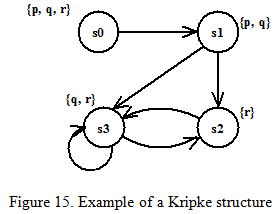
\includegraphics[width=40mm]{Kripke.png}
%{CTL not in LTL.jpg}}
}}
{\vspace{-0cm}
\visible<3->{
\begin{example}[CTL not in LTL]
 A G E F (brake == true)
\end{example}}
\visible<4->{
Two systems have the same sets of traces but only one satisfies the formula in CTL.}
}}
{
\begin{example}[LTL not in CTL]
A F G (black = true)\\
For all runs there will be a moment from which onward holds
(black = true).
\visible<7->{The idea is to construct two sequences of systems $T_i$ and $T_i'$
such that:} 

\begin{enumerate}
\item<7-> $(T_i,s_0)\models A F G (black = true)$ but
    $(T_i',s_0)\not\models AF G (black = true).$ 
\item<7-> $(T_i,s_0)$ and $(T_i',s_0')$ are not distinguished by any CTL formula of the modal depth $i$.
\end{enumerate}
\end{example}

\visible<8>{Look: \url{https://www.youtube.com/watch?v=OAf7q3X71-o}
(min 58)}
}
}}}
\end{frame}

\begin{frame}{Proof.}
\Margines{
\DwieKol{0.45}{0.40}{\  

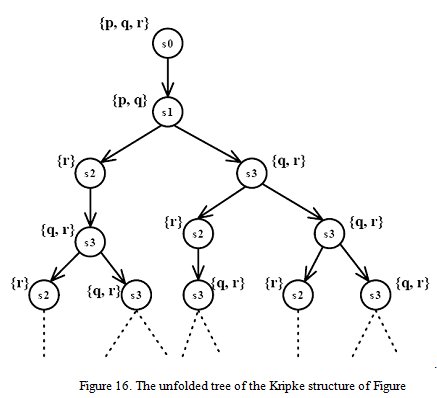
\includegraphics[width=50mm]{UKripke.png}
}{\alt<2>
{Let $\sim_i$ not distinguishable by CTL formulas of depth $i$.
\begin{proof}[$T_i\sim_i T_i'$]
Via induction on $i$, ( the size of the formula).

   Induction hypothesis: 
    $T_k\sim_i T_j'$ 
    for $i\leq k\leq j$.

\end{proof}
}
{Let $\sim_i$ not distinguishable by CTL formulas of depth $i$.
   \begin{lemma}[Auxiliary]
    $P_i\sim_i P_j$ for $i\leq j$.
    $R_i\sim_i R_j$ for $i\leq j$.
   \end{lemma}
   \begin{proof}
   Via induction on $i$, ( the size of the formula).
   
   Induction hypothesis: 
    $P_k\sim_i P_j,$ 
    $R_k\sim_i R_j$ 
    for $i\leq k\leq j$.
   \end{proof}
   }
}}   
\end{frame}


\begin{frame}{Comparison table}
\Margines{
\begin{center}
\scriptsize
\renewcommand{\arraystretch}{1.35}
\resizebox{\textwidth}{!}{%
\begin{tabular}{|l|c|c|c|}
\hline
 & LTL & CTL & CTL* \\
\hline
Formulas evaluated in & paths / traces & states & states and paths \\
\hline
Path quantifiers & implicit universal & explicit \(A,E\) & explicit \(A,E\) \\
\hline
Time view & linear & branching & branching + linear \\
\hline
Typical algorithm & \Buchi\ automata & state labelling & automata / tableaux \\
\hline
Model checking & PSPACE in formula & linear-time explicit & PSPACE in formula \\
\hline
\end{tabular}}
\end{center}

\begin{block}{Practical rule}
Use LTL for properties of complete executions. Use CTL when the existence or inevitability of future choices matters explicitly.
\end{block}
}
\end{frame}

\begin{frame}{Summary}
\Margines{
\begin{itemize}
  \item LTL specifies properties of infinite traces over \(\Sigma=2^{\AProp}\).
  \item LTL model checking can be reduced to \Buchi\ automata emptiness.
  \item CTL adds explicit path quantifiers \(A\) and \(E\).
  \item CTL model checking can be performed by computing satisfying states bottom-up.
  \item CTL* contains both CTL and LTL, but is syntactically and algorithmically heavier.
  \item LTL and CTL are not comparable: each can express properties that the other cannot.
\end{itemize}
}
\end{frame}



\begin{frame}{Bibliography}
\Margines{
\begin{itemize}
  \item Christel Baier and Joost-Pieter Katoen, \emph{Principles of Model Checking}, MIT Press, 2008.
  \item Edmund M. Clarke, Orna Grumberg, and Doron A. Peled, \emph{Model Checking}, MIT Press, 1999.
  \item Moshe Y. Vardi, automata-theoretic approach to LTL model checking.
  \item Supplementary videos: Units 3--8 from\par
  \url{https://www.youtube.com/channel/UCUXDMaaobCO1He1HBiFZnPQ/videos}
\end{itemize}
}
\end{frame}





\end{document}
